\chapter[Long-term Semantic OS using changes in the organisation of the environment over time]{Long-term Semantic OS using changes in the organisation of the environment over time}%Temporal Semantic OS system based on heat maps
\label{chap:4_temporal_os_system}
\section{Introduction}
\label{sec:introduction}
We have already seen the advantages of using organisational semantic information in OS results. The early semantic information is inferred from both the organisation of door signs and the corridors of a building, which rarely change over time. In most of the time, rooms are identified by signs that last for many years, as well as the corridors that are only changed when the environment goes through a renovation. Our previous OS system, NSOS~\cite{Mantelli2021Semantic}, Chapter~\ref{chap:3_text_os_system}, estimates the organisation of indoor environments for OS tasks based on static source of data to infer the organisation semantic information. However, it is no surprise that SRs sometimes operate in semi- and fully-dynamic environments, where some objects and obstacles move occasionally, e.g. chairs in the launch area, or very often, e.g. front doors of a building. Once the SR robot has found the room that it was looking for, and it has to interact with some objects within such a room, it would be interesting that the robot could efficiently search for them. In this chapter we discuss how an OS system could estimate the organisation of the environment even if it is not static as in the previous chapter. 


%A considerable amount of innovative mobile ground robots have been designed recently~\cite{Portugal2021Improving}. This is partially motivated by their use in indoor and human-centered environments, in which the International Organization for Standardization defines them as service robots~\cite{Lu2020Service, ISO8373}. Furthermore, 
%copiei daqui
%the increasing number of older people living at home supports the need for service robots to automate processes and tasks that may be tedious, inconvenient, or even challenging for older people~\cite{Paulius2019Survey, Torresen2020Special}. 

%In general, service robots can contribute on practical tasks for humans as robot assistants or robot companions, such as watching older adults with regard to emergency situations, reminding people to take their medicines, and searching, picking, and placing objects~\cite{Paulius2019Survey, Torresen2018Robot, Sprute2017Ambient}. 
%até aqui
%The specific task of searching for objects is harder for older adults than for younger ones, and it illustrates how service robots can be a helpful tool. This task is challenging because the elderly are more likely to suffer from impaired memory, and hence the chances are higher for them to forget where a specific object is placed. Therefore, they might spend a considerable amount of time and energy searching for it, besides risking their health due to the possible mobility restrictions. Likewise, young people also aim to save time and energy in searching tasks, even if they are healthy and capable of walking for long distances~\cite{Sprute2017Ambient}. Therefore, mobile ground service robots are a convenient tool to assist people in OS tasks and many more, either in large indoor environments for young people, such as offices and factories, or in small indoor environments for older adults, like their own houses or care centers. 

%Although a brute-force OS strategy seems a straightforward solution, it does not efficiently solve the problem. It will eventually find the target object, but the searching process may be time-consuming due to the long distances traveled by the robot~\cite{Rasouli2020Attention}. Therefore, it is important to consider a search strategy incorporating different information from both the environment and the objects, to improve the searching performance. %An efficient search strategy cuts down the problem's searching space, thus preventing the robot from traveling long distances.

%The research community has explored the advantages of different sensors in the OS field, and except for the proposed works that focused on the robot's perceptual limitations~\cite{Cabanillas2010Efficient, Lopez2008Hybrid, Deyle2014Finding}, the majority of them are based on visual sensors. This is because visual sensors are becoming cheaper and smaller without compromising the data quality, which is suitable for robotic applications. Besides, the large variety of data they provide, e.g., RGB-D images and point clouds, encourages the researchers to propose OS strategies based on different information, such as objects' color~\cite{Chen2013Visual}, texture and shape~\cite{Meger2010Curious}, and even their category provided by an object detection algorithm~\cite{Forssen2008Informed}. 

%Similar to the task of human-object interaction in Computer Vision, which infers the relationship between humans and objects, we assume that human activities have an influence in the objects' placement~\cite{Zhou2020Cascaded}. Hence, we argue that a robust OS strategy  should also consider the semantic information of how a human interacts with the objects throughout a period of time, rather than only the object's shape or color. Instead of filtering the changes within the environment, the OS approach could model and incorporate the object's position changes to make predictions about its future positions~\cite{Krajnik2020Chronorobotics}. For example, a person may move their smartphone many times throughout a day, but there are high chances of being on the bedside table during the night. Suppose the robot is tasked with finding the smartphone at night, and the OS approach can understand this pattern. In that case, it will reduce the searching space to a few regions of the bedroom and hence, improve the robot's overall performance. 

%Besides, an approach that relies on such semantic information, i.e., human-object interaction, can incorporate someone's habits regarding how they usually place the objects. For example, imagine a person that is used to place a mug on top of the sofa's arm or on the coffee table, both places in the living room. An OS system that relies on the association of rooms to specific objects (e.g., kitchen and plates or bedroom and pillows) to prioritize the searching would probably start the process in the kitchen instead of the living room~\cite{Aydemir2013Active, Wang2018Efficient}. On the other hand, a strategy based on the human-object interaction would understand the particularities of the place in which the service robot operates, i.e., the human's habits and routine, regardless of whether it makes sense for most people, e.g., looking for a laptop in the kitchen.

\subsection{Proposal and contributions}
\label{subsec:chap4_proposal_contributions}
In this chapter, we propose a Long-term Semantic OS system (LSOS) that estimates which regions of the dynamic environment are more promising to find a target object. The search is based on how the organisation of objects throughout a period of time. We assume that human activities have an influence in the objects' placement~\cite{Zhou2020Cascaded}. Besides, we argue that a robust OS strategy should consider the semantic information of how humans interact with objects over time, rather than searching object only based on their shape or color. Instead of filtering the changes within the environment, the OS system could model and incorporate the changes in the object's position to make predictions about its future positions~\cite{Krajnik2020Chronorobotics}. For example, a person may move their smartphone many times throughout a day, but there are high chances that it will be on the bedside table during the night. Suppose the SR is tasked with finding the smartphone at night, and the OS approach can understand this pattern. In that case, it will reduce the regions to search for only the bedroom. Consequently, it would improve the robot's overall performance during the search. 

Our LSOS system works in two modes. One is called recording, and it collects objects' data in the unknown environment, whereas the other is called requesting, and it is responsible for processing the saved data to perform the search. In the recording mode, the SR gathers information about the surrounding objects over a period of time, and then it builds the map of the environment (or just update it in case it already exists). The mapping could be done while the SR carries out other tasks, such as cleaning the floor or watching an older person. The requesting mode is executed when someone requests the SR to find a target object, in which our LSOS processes the gathered data to estimate where the object might be at the request moment. We use a Heat map to represent the probability of finding the target object, in which areas where are more likely to have the target object located are more heated than elsewhere. Before we continue, it is important to highlight that in the previous chapter our NSOS actually searched for objects and not just numbers from door signs. The numbers are the identifying code for the doors, which were real object that our NSOS system meant to find and that the numbers were associated with. Therefore, even though the numbers of the door signs may not be a real object, in the end our previous NSOS system was searching for an object, as our next LSOS system does. The diference is that NSOS searcher for only one type of object, doors, whereas LSOS can search for different sorts of objects, as we will see in this chapter.

Figure~\ref{fig:intro_general_idea} illustrates how the core of our LSOS system, the requesting mode, works. For this example, imagine that a SR has already moved through the whole area performing the recording mode. Then, it built the 2D grid map and recorded the location of objects and the hour they have been detected. Saving the detection hour of an object, along with its position, is the core of our LSOS system. By doing this, our system will be able to estimate the organisation of the objects over time in the environment, and efficiently find the target object. It is as if the system could learn the the objects arrangement in different moments of the days, and recognise patterns. Back to the example, when the SR receives a request to find a mug at 14:00, as shown in Figure~\ref{fig:intro_general_idea}, our the requesting mode of LSOS uses the recorded information that a mug has been detected twice. The first time, at 9:00, it was in region A, and it was moved to region B at 13:00. The recording mode compares the current time, 14:00, with the two detection hours of the object. Then, it decides which region it should start searching. As region B has the smallest difference to the querying time, i.e. the most recent time the object has been seen it was in region B, the robot goes to that region first. The idea is that the more data our LSOS records, the more precisa are its estimations.

\begin{figure}[h]
    \centering
    \includegraphics[width=.8\textwidth]{figs/general_idea_300dpi.png}
    \caption[One example of our proposed LSOS system operating in our custom made simulated environment.]{One example of our proposed LSOS system operating in our custom made simulated environment. The robot's task is finding a mug at 14:00.}
    \label{fig:intro_general_idea}
\end{figure}

The contributions of our this chapter are presented below: 
\begin{itemize}
\item \textbf{OS system}: a probabilistic OS system that does not require a priori map from the environment, a training phase, nor data annotation. It builds a 2D grid map of the environment to estimate the robot's pose and indicate the free cells regions for navigating. Simultaneously, it builds a Heat map based on the 2D grid map, representing the computed estimations of the object's likelihood for each area. For our LSOS system, a 3D map would not be favorable, as its benefits do not make up for the computational cost of building and updating it. A simple 2D is already suitable for our LSOS needs. 
\item \textbf{Self-contained OS system}: a semantic OS system that works independently. It does not depend on a specific SLAM system for mapping the environment or an object detection module for detecting the objects. It only requires the robot's and object's pose within the map, the object's class, and the hour in which detection happened, which will be stored during the recording information mode.
\item \textbf{Semantic, temporal OS strategy}: a new strategy for OS that takes advantage of the organisational semantic information inferred from the objects arrangement throughout a period of time. It aims to reduce the amount regions of the environment that the SR has to search in, and improve the overall results. It saves information about \textit{when} the objects were \textit{where}, and then estimates the map regions' likelihood of containing the target object.
\item \textbf{Advantages of the organisational semantic information}: in contrast to most of the works in robotics, which assume the world is static and filter the dynamic agents, our LSOS system incorporates the changes in the objects' position in the environment to improve the robot's performance in OS tasks. We present an analysis of the advantages of using such type of information as input to our system, which permits an efficient estimation of the region which is more likely to contain the target object. 
\end{itemize}

%The remainder of this work is organized as follows. Section~\ref{sec:relatedwork} reviews the literature and discusses the works that propose OS approaches and the ones that deal with long-term in robotics. After briefly describing our temporal, semantic OS system in Section~\ref{sec:system_overview}, we dive deep into it in Section~\ref{sec:semantic_strategy} and explain all the details from our system and our custom model for Yolo. Next, Section~\ref{sec:experiments_results} introduces the experiments, both in simulation and with the HH106 dataset. In the simulation, we compared our system against two other ones in the same scenario, an eleven-room indoor environment. The HH106 dataset contains human presence data collected over two months. It was adapted to the OS task context in which our OS system estimated the human's position at different times. Lastly, Section~\ref{sec:conclusion} concludes this work, summarizing the contributions and proposing future works.

\section{LSOS System Overview}
\label{sec:cap2_system_overview}

Our LSOS system is based on spatio-temporal information, and it requires data from the past to perform OS tasks efficiently. It is important to highlight that  although our LSOS system depends on previous observations of the objects to compute the estimations, no data must be provided to LSOS \textit{a priori}. Nevertheless, that is the only requirement of our system. The more observations the recording mode saves, the more precise are the estimations from the requesting mode. Our LSOS system does not depend on ambient sensors like in~\cite{Sprute2017Ambient} or environmental changes. Even though smart houses may have visual sensors that could be used to expand the SR's FoV, an OS system that depends on such set of sensors restricts its usage in other regular houses. Therefore, we focused on making our LSOS system self-sufficient, resulting in a two-mode recording and requesting system. Besides, our system can run simultaneously with any other task the SR performs, such as cleaning the environment or monitoring an old adult. Hence, a single SR can perform multiple tasks along with our LSOS system. Further, it does not require any changes in the environment, such as mounting cameras in different rooms.

\begin{figure}[h]
    \centering
    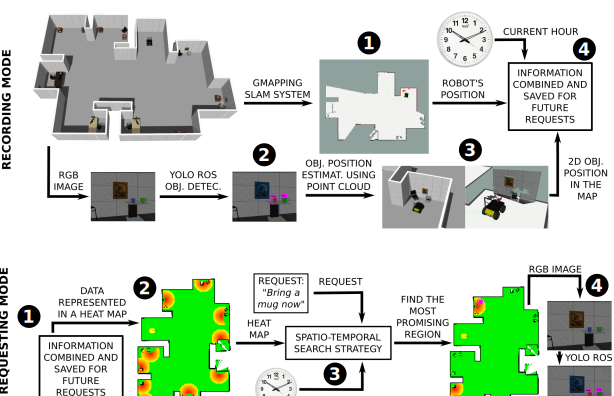
\includegraphics[width=1\textwidth]{figs/system_overview.png}
    \caption[Flowchart that explains how our LSOS system works.]{Flowchart that explains how our LSOS system works. The top half is the mode in which the robot gathers information about the environment, and the bottom half is the one that is executed when the robot is active with finding an object.}
    \label{fig:system_overview}
\end{figure}

The first mode, recording, is responsible for gathering and saving all the data that our LSOS system needs, as the upper half of Figure~\ref{fig:system_overview} illustrates. The goal of this mode is to fulfill our OS system's requirements, as mentioned earlier. The more data it gathers from the environment, the more efficient our OS system becomes. In summary, the recording mode relies on an object-detection algorithm and a SLAM system. We use YOLO for object-detection (see Chapter~\ref{chap:2_you_only_look_once}), as it is a robust and popular package for such task, and apply the Gmapping package, a laser-based SLAM for building a 2D grid map~\cite{Bjelonic2018Yolo, Gerkey2020Gmapping}. 
During the execution of this mode, when an object is within the camera's point of view, YOLO detects it.  A depth camera with a point cloud measures the distance between the robot and the object, and then our system calculates its position in the map given the robot's pose. Once the robot's and object's position are known, our system saves this information, along with the detection hour and the class of the object provided by YOLO. This recording mode can be executed hourly, daily, or while the robot performs any other task. It is also important to highlight that our OS system is not restricted to YOLO and Gmapping. Any object-detection and SLAM package, respectively, provide the same data type our system saves, and hence, could be used in our system. 

The second mode, requesting, is performed by our LSOS system when the robot is active with finding an object, i.e., when someone requests it to look for a target object. It worth to mention that when when our system is requested to search for a target object, it does not differentiate the instances of that object. For example, when searching for a book, both \textit{The Lord of the Rings} and \textit{Don Quixote} (and any other book) are valid options to LSOS. Hence, the target object represents a class of objects, and finding any instance that belongs to that class is sufficient. Furthermore, this mode aims to find the target with the robot traveling the shortest distance to save time and the robot's resources. All the data gathered in the recording mode plays an important role here, as it helps to improve the estimations of our LSOS system. The more data the recording mode records, the better is the estimation computed by the requesting mode. The lower half of Figure~\ref{fig:system_overview} illustrates the entire requesting process. The requesting mode builds a heat map out of the recorded data to estimate which environment regions are more promising to locate the target object in. In contrast to many OS systems in the literature, our proposal considers the hour that objects have been detected and compares them with the request hour. Therefore, when the robot receives a request, it goes to the warmest spot in the heat map, i.e., region of the environment where is more liley to find the target object. Lastly, if the requesting mode is executed before the recording one, and no data from the environment is available, our OS system would perform a brute force search since no information is available to improve its performance.

Although our LSOS system makes predictions based on the arrangement (organisation) of objects, it does not have a separate training phase to learn the objects' presence, like machine learning algorithms.
In fact, both modes (recording and requesting) can run in parallel, albeit the more information the map contains prior to the search, the better the search results tend to be. Another important point is that the semantic map in which the searches are based is not a black box. On the contrary, it relies on a probabilistic approach that infers the most promising regions to find the target object by recording how people interact with it. Besides, as the experiments presented below suggest, a small amount of data is enough for our system to succeed.

\section{Our LSOS system's search strategy}
\label{sec:semantic_strategy} 
This section details our OS system and how it works. It starts with the description of the heat map module in Sections~\ref{subsec:heat_map} and ~\ref{subsec:inverting_kernel}, with explanation of how our LSOS system builds it based on the gathered data in the recording mode. Finally, Section~\ref{subsec:final_formula} presents the goal computation, which explains how our OS system estimates the most promising map regions to find the target object, i.e., the warmest spots in the heat map. It also discuss how our OS system behaves when the object is not found at the most promising region of the map.

%\subsection{Custom object detection model}
%\label{subsec:custom_obj_detect_model} 
%TO DO by Farzan

\subsection{The Heat Map and the representation of the objects' presence}
\label{subsec:heat_map}
The heat map is a visual technique widely used for visualizing complex spatial patterns, proposed by Kinney~\cite{Kinney1993Heatmaps}. It provides a meaningful and straightforward understanding for humans and processing programs. In this chapter, the discrete distribution of objects' presence is processed into a continuous color distribution, in which the most likely regions to find the target object are intuitively revealed. 

The 2D grid map $\bs{m}$ that has been built by the SLAM system during the recording mode is used for computing the heat map~$\bs{h}$. Both maps are equal in terms of the number of cells and size, but the difference is that a cell $\bs{m}_i \in \bs{m}$ is either free, occupied, or unknown, whereas the same cell $\bs{h}_i \in \bs{h}$ is the heat value that represents how likely that location is to contain a certain object. A cell in both $\bs{m}$ and~$\bs{h}$ represents exactly the same place in the environment. Hence, only the cells that are either free or occupied in $\bs{m}$ are likely to have a heat value different than zero in $\bs{h}$, as there are no objects on unknown regions in~$\bs{m}$.

All the~\textit{n} objects that have been detected in the recording mode are represented by the set $\mathbf{O}$, in which $\mathbf{O} = \{\bs{o}_1, \bs{o}_1, \cdots, \bs{o}_n\}$. Each $\bs{o}_j \in \mathbf{O}$ is composed by its position within~$\bs{h}$, its class, the hour it has been detected, and the robot's position during the detection, i.e., $\bs{o}_j = (\bs{o}_j^p, \bs{o}_j^c, \bs{o}_j^h, \bs{o}_j^r)$, respectively. To compute~$\bs{h}$, we represent the presence of the object $\bs{o}_j \in \mathbf{O}$ by a weighted circular kernel $K(\cdot)$ of radius~\textit{r}. Let~\textbf{T} be the set of cells within the area of $K(\cdot)$ for a given~\textit{r}, and $\mathbf{T} \in \bs{h}$. For all cells $\bs{h}_i \in \mathbf{T}$, $K(\cdot)$ is defined as
\begin{equation}
K\big(D(\bs{h}_i,\bs{o}_j^p), \bs{o}_j^h\big) = 
  \begin{cases}
 W(rh, \bs{o}_j^h)Q(\bs{h}_i)(1 - \frac{d}{r}), & \quad  $if$~d \leqslant~r\\ 
 \hfill 0,  & \quad~$otherwise$
  \end{cases}    
\label{eq:kernel_definition}
\end{equation}
where~$D(\bs{h}_i,\bs{o}_j^p)$ is the Manhattan distance from the current cell being measured, $\bs{h}_i \in \mathbf{T}$ to the centre of the kernel, $\bs{o}_j^p \in \bs{h}$. The function $Q(\cdot)$ is defined as
\begin{equation}
Q(\bs{m}_i) = 
  \begin{cases}
    0, & \quad \text{if}~\bs{m}_i~\text{is unknown in }\bs{m}\\ 
    1, & \quad \text{otherwise}
  \end{cases} 
\label{eq:q_function_unknown_cells}  
\end{equation}
and it checks whether a cell $\bs{m}_i$ is unknown in $\bs{m}$. The other function $W(rh, \bs{o}_j^h)$ computes the difference between the hour the object has been detected, $\bs{o}_j^h$, and the hour the robot is requested to perform the search, $rh$. This difference is then used to compute the weight factor of the object $\bs{o}_j$, since the smaller is the hour difference, the more important that object becomes to the search. This function is defined as
\begin{equation}
W(rh, \bs{o}_j^h) = 1 - \frac{\left | rh - \bs{o}_j^h \right |}{12} 
\label{eq:hour_weight}
\end{equation}
Here is important to mention that we use the 24-hour notation. Hence, $W(rh, \bs{o}_j^h)$ is equal to one when $rh$ and $\bs{o}_j^h$ are equal, and it is zero when they are 12 hours apart from each other, i.e., the largest difference in hours between two different time stamps. 
%In this chapter, Equation~\ref{eq:hour_weight} computes the weight of the object $\bs{o}_j$, in which the closer both hours are, the more important the object becomes for the search. 
For example, if ou LSOS system detected an object two times, at 8:00 in position A and 14:00 in position B, and it is performing the search at 10:00, it will probably start searching the object in A, as 8:00 is closer to 10:00 than 14:00.

The first part of computing the heat map~$\bs{h}$ is depicted in Figure~\ref{fig:kernel_heat_map}. 
%The map of the environment in simulation is illustrated in Figure~\ref{fig:kernel_heat_map}-(a), and in Figure~\ref{fig:kernel_heat_map}-(b) the map~\textbf{M} is presented. 
The outcome of Equation~\ref{eq:kernel_definition} is shown in Figure~\ref{fig:kernel_heat_map}c, in which every object from~\textbf{O} is represented by the kernel $K(\cdot)$. It is important to notice that the warmest cells in~$\bs{h}$, Figure~\ref{fig:kernel_heat_map}c, are at the objects' positions in Figure~\ref{fig:kernel_heat_map}a. 

\begin{figure}[!h]
\centering
\includegraphics[width=.8\textwidth]{figs/environment_2Dgrid_heatmap_kernel.png}\\
(a)\hspace{2.8 cm}(b)\hspace{2.8cm}(c)
\caption[Example of the computed heat map given a set of detected objects.]{Example of the computed heat map given a set of detected objects. (a) is the simulated environment with 10 objects spread in seven rooms. (b) is the 2D grid map built by Gmapping. (c) is the heap map built by our OS system, considering the map in (b) and the detected objects in (a). The warmer regions represent their position within the map.}
\label{fig:kernel_heat_map}
\end{figure}

The computed heat map $\bs{h}$ in Figure~\ref{fig:kernel_heat_map}c indicates which regions our LSOS system should search, since it does not consider the colder spots (green region) in~$\bs{h}$. Besides, the class of an object helps to focus the searching in more promising regions, as there is no point in searching in a warm spot where there is only a book if our system is looking for a mug. Since the class of a detected object $\bs{o}_j$ is known, $\bs{o}_j^c$, our system ignores warm spots from objects with different classes than the target one.

A third adjustment in the process of computing the heat map comes with a subtraction on the circular kernel's angle. During the search, our OS system guides the robot towards the edge of the most promising kernel. The edge, yellow cells  in~$\bs{h}$, is one of the best regions to place the robot because it is the ideal distance between the robot and the kernel center (or the object's position). However, despite the ideal distance, positioning the robot at any place over the edge of the kernel does not ensure the object will be either recognised or even within the camera's field of view. This issue is illustrated in Figure~\ref{fig:bad_robot_placement}, in which the robot is quite close to the compute monitor at the edge of its kernel, but yet the object detection module is not able to detect it. Alternatively, the most appropriate position to place the robot would be the same one that the robot has been in when recognizing the object during the recording mode. Thus, it is most likely that the object detection module will recognize the object once again if the robot assumes a similar pose it has assumed before. Hence, our heat map~$\bs{h}$ is built considering the kernel $K(\cdot)$ in Equation~\ref{eq:kernel_definition} with an acute angle, instead of considering a \ang{360} one. For a given object~$\bs{o}_j$, its kernel's angle is defined considering its robot's position when it has been recognised, i.e., $\bs{o}_j^r$. Figure~\ref{fig:good_robot_placement} illustrates the advantage of restricting the kernel's angle, in which the object detection module recognize the computer monitor.

\begin{figure}[!h]
\centering
\includegraphics[width=.6\textwidth]{figs/bad_robot_placement_1.png}\\ 
(a)\hspace{3.5cm}(b)
\\
\includegraphics[width=.6\textwidth]{figs/bad_robot_placement_2.png}
\\(c)\hspace{3.5cm}(d)
\caption[Example of the robot at the edge of the kernel, and yet not recognising the object.]{Example of the robot at the edge of the kernel, and yet not recognising the object. (a) is the environment in simulation, (b) is the robot in $\bs{m}$, (c) is the robot in~$\bs{h}$, and (d) the current image capture by the robot's camera. %Even though the robot is considerably close to the computer monitor, the object detection module can not detect it due to the point of view.
}
\label{fig:bad_robot_placement}
\end{figure}

\begin{figure}[!h]
\centering
\includegraphics[width=.6\textwidth]{figs/good_robot_placement_1.png}\\
(a)\hspace{3.5cm}(b)
\\
\includegraphics[width=.6\textwidth]{figs/good_robot_placement_2.png}
\\(c)\hspace{3.5cm}(d)
\caption[Example of the modified kernel with an acute angle, and the recognised object.]{Example of the modified kernel with an acute angle, and the recognised object. (a) is the environment in simulation, (b) is the robot in $\bs{m}$, (c) is the robot in~$\bs{h}$, and (d) the current image capture by the robot's camera. %It is possible to note that the robot's current position is suitable for recognizing the object since it is similar to the one the robot had assumed before when the object was recognised for the first time.
}
\label{fig:good_robot_placement}
\end{figure}

The adjustments performed while computing the heat map~$\bs{h}$ plays an important role in our LSOS system. Figure~\ref{fig:step_by_step_search_space_reduction} represents the step by step of each adjustment, and the outcome is a few warmer spots in~$\bs{h}$. Besides saving computational resources by reducing the amount of regions to search, there is also an increase in the chances of detecting the target object by the proper robot positioning. 

\begin{figure}[!h]
\centering
\includegraphics[width=.9\textwidth]{figs/step_by_step.png}\\
(a)\hspace{3cm}(b)\hspace{3cm}(c)\hspace{3cm}(d)
\caption[Step by step of the space reduction performed by our OS system.]{Step by step of the space reduction performed by our OS system. (a) is the empty~$\bs{h}$, (b) is the representation of all objects from~\textbf{O} with the circular kernel $K(\cdot)$, (c) is the kernels' angle reduction given the robot's position of each object, and (d) is the outcome of considering only objects with the same class as the target's one and the other ones are ignored.}
\label{fig:step_by_step_search_space_reduction}
\end{figure}

\subsection{Inverted kernel $IK(\cdot)$}
\label{subsec:inverting_kernel}
Our system performs another operation to make it easier to find the target object. In OS systems, one of the main goals is to place the robot at the most appropriate place to accomplish the task. In this chapter, as we already mentioned, the most promising regions to place the robot are at the kernels' edges due to the ideal distance to the objects. However, such edges in the kernel $K(\cdot)$ presented in Equation~\ref{eq:kernel_definition} are the coldest regions within the kernel area, as the warmest one is at the kernel's center. Hence, if our system computes the inverse $IK(\cdot)$, the warmest regions becomes the ones at the edge, i.e., the ideal spots to place the robot during the search are the ones with the highest heat value. The $IK(\cdot)$ is similar to the one presented in Equation~\ref{eq:kernel_definition}, and it is defined as

\begin{equation}
IK\big(D(\bs{h}_i,\bs{o}_j^p), \bs{o}_j^h\big) = 
  \begin{cases}
 W(rh, \bs{o}_j^h)Q(\bs{h}_i)\frac{d}{r}, & \quad  if d \leqslant~r\\ 
 \hfill 0,  & \quad \text{otherwise}
  \end{cases}    
\label{eq:inverse_kernel} 
\end{equation}

In summary, the difference between Equations~\ref{eq:kernel_definition} and~\ref{eq:inverse_kernel} is that the former computes~$\bs{h}$ as the warmer regions being the object's position, whereas the latter computes~$\bs{h}$ as the warmer regions being the ideal place to position the robot during the search. Figure~\ref{fig:different_kernel_comparison} shows their difference. 

%\begin{figure}[!h]
%\centering
%\hspace{.4cm}(a)\hspace{2.6cm}(b)\\
 %\rotatebox{90}{\hspace{1cm}\text{Circular kernel}}
 %\includegraphics[width=.5\textwidth]{figs/normal_inverse_kernels_complete.png}\\
 %\rotatebox{90}{\hspace{1cm}\text{Reduced kernel}}
 %\includegraphics[width=.5\textwidth]{figs/normal_inverse_kernels_reduced_angle.png}
%\caption{The difference between the kernel and its inverse. (a) is the kernel presented in Equation~\ref{eq:kernel_definition}, in which its center is the warmest spot. (b) is the inverse kernel, defined by Equation~\ref{eq:inverse_kernel}, in which the inverse kernel's edge are the warmest spots. (a) intuitively represents the object's presence, whereas (b) represents the best places to position the robot to find a target object.}
%\label{fig:different_kernel_comparison}
%\end{figure}

\begin{figure}[!h]
\centering
  Normal kernel\hspace{4.5cm}Inversed kernel\\
  \vspace{.3cm}
 \includegraphics[width=.45\textwidth]{figs/normal_kernel_complete_reduced.png}
 \includegraphics[width=.45\textwidth]{figs/inversed_kernel_complete_reduced.png}\\
 (a)\hspace{3cm}(b)\hspace{3cm}(c)\hspace{3cm}(d)

\caption[The difference between the normal kernel and its inverse.]{The difference between the normal kernel and its inverse. (a) and (b) represent the normal kernel, the circular and reduced version, respectively. (c) and (d) represent the same for the inversed version of the same kernel.}
\label{fig:different_kernel_comparison}
\end{figure}

Despite the easy readability by humans of~$\bs{h}$ built by Equation~\ref{eq:kernel_definition}, due to the intuitive object's presence representation, for our OS system Equation~\ref{eq:inverse_kernel} provides the most appropriate~$\bs{h}$. Therefore, for now on, all references of~$\bs{h}$ within this work considers that it has been built using Equation~\ref{eq:inverse_kernel}.

\subsection{Goal computation in the request mode}
\label{subsec:final_formula}

The process of building the heat map~$\bs{h}$ and reducing the search space is the first part of our OS system, in which we represent the data from the recording mode in~$\bs{h}$. In addition to that, it is also necessary to compute the goal, i.e., the most promising spot in~$\bs{h}$ that our system estimated to the robot go and find the target object. This computation is performed when the robot is requested to look for the target object.%In Figure~\ref{fig:step_by_step_search_space_reduction}-(d), for example, the goal would be one of the two remaining warm spots since they represent objects with the category than the target one. 

The goal computation is similar to the heat map construction because we also use a kernel approach. Our idea here is to analyse the whole~$\bs{h}$ in several circular kernels, and get the cell $\bs{h}_i^*$ that neighbours have the highest probability of containing the target object, $\bs{o}_j$, for the request hour, $rh$. The final equation for computing the goal cell $\bs{h}_i^* \in \bs{h}$ is defined as
\begin{equation} 
\bs{h}_i^* = \underset{\bs{h}_i\in\bs{h}}{\text{arg max}}\big(\varphi(\bs{h}_i, \bs{o}_j, rh)\big)    
\label{eq:final_equation}
\end{equation}
in which the function $\varphi(\bs{h}_k)$ computes the possibility of the cell $\bs{h}_i$ contains the target object, $\bs{o}_j$. It is defined as
\begin{equation}
\varphi(\bs{h}_k,\bs{o}_j, rh) = \sum_{\bs{h}_i}^{\mathbf{T}}H(\bs{h}_i,\bs{o}_j, rh)
\label{eq:psi_function}
\end{equation}
where $\mathbf{T}$ is a set of cells within the kernel area and $\mathbf{T} \subset \bs{h}$ centred in $\bs{h}_k$. The function $H(\cdot, \cdot, \cdot)$ returns the heat value (or probability) of the target object $\bs{o}_j$ being in the cell $\bs{h}_i$, at the request hour, $rh$.


%and $K'(\cdot)$ is a simpler version of the kernel presented in Equation~\ref{eq:kernel_definition} defined as
%\begin{equation}
%K'(d) = 
%  \begin{cases}
% a, & \quad  \text{if~}d\leqslant r\\ 
% \hfill 0,  & \quad \text{otherwise}
%  \end{cases} 
%\label{eq:kernel_goal}
%\end{equation}
%$r$ is the radius of $K'(\cdot)$, different from the one used in Equation~\ref{eq:kernel_definition}, and~\textit{d} is the Manhattan distance. 

It is possible that for a certain request to our OS system, there are multiple regions in~$\bs{h}$ that register the presence of instances of the target object. Thus, our OS system computes Equation~\ref{eq:final_equation} over~$\bs{h}$ and sorts the multiple $\bs{h}_i^*$ according their likelihood. The robot is moved towards the most likely one, and if the target object at that position is not found, the robot proceeds to the second most promising $\bs{h}_i^*$. This process is repeated until the robot visits all regions that register the presence of the target object. Lastly, in the worst case where the object was not found in any promising regions, the robot inspects all unvisited rooms, similar to a brute force search.

\section{Experiments and Results} 
\label{sec:chap2_experiments_results}
This section is divided into four subsections. %Section~\ref{subsec:object_detection_module} presents the experiment with Yolo, comparing our customized model with the standard ones publicly available. 
Section~\ref{subsec:datasets_simulation} discusses the dataset and simulation setup used throughout the experiments. Section~\ref{subsec:comparison_approaches} explains the other two OS systems that we compare against our proposal, followed by Section~\ref{subsec:simulated_experiment_setup} that presents the experimental setup to which the three OS systems have been tested, along with their respective performances. Section~\ref{subsec:hh106_dataset} shows the performance of our LSOS system in estimating the person's presence given the HH106 dataset.

%\subsection{Object detection module}
%\label{subsec:object_detection_module}
%The Yolo object detection system can be either used with a pre-trained model, in which the Yolov2 and Yolov3 are the most popular models, or with a new customized one. This experiment aims to measure the Yolov2, Yolov2-tiny, and Yolov3's efficiency against our customized one, in detecting objects in the simulation. We have created the scenario illustrated by Figure~\ref{fig:darknet_experiment}, in which the robot follows the red path, autonomously visiting all the three objects, computer monitor, book, and mug. The robot remains still in front of each object for seven seconds, and then it continues to the next one. We collect the data about each model's performance only within these seven seconds.
%
%The performance of each model was measured by its FPS rate, object prediction accuracy, and recall. The experiment was repeated five times for each model, with the robot starting at the same position in every run, and Table~\ref{tab:darknet_experiment} presents the results. As each model was repeated five times, we calculated the recall of each model while detecting every object, along with the average of the detection belief from the correct detections. If a model failed to recognize the object in a run, we considered the prediction accuracy for that object as zero.
%
%\begin{figure}[!h]
%\centering
%\includegraphics[width=.7\textwidth]{figs/darknet_experiment_edited.png}
%\caption[The setup in simulation for the experiments with different models for Yolo.]{The setup in simulation for the experiments with different models for Yolo.}
%\label{fig:darknet_experiment}
%\end{figure}
%
%\begin{table*}
%\centering
%\caption[Performance of each tested model tested in our experiment with Yolo.]{Performance of each tested model tested in our experiment with Yolo.}
%\begin{tabular}{cc|ccc}\toprule
%\multicolumn{2}{c|}{\textbf{Yolo's models}} & \multicolumn{3}{c}{\textbf{Objects}}\\
%\textbf{Name} & \textbf{Data} & \textbf{Comp. Monitor} & \textbf{Book}    & \textbf{Mug}  \\\midrule
%\multirow{3}{*}{YoloV2-tiny} & Acc. Aver. & 46.0~$\pm$~0 & 45.50~$\pm$~7.78 & 64.20~$\pm$~8.70
%\\
% & Recall & 20\% & 40\% & 100\%\\
% & FPS & 12$\sim$160 & 12$\sim$160 & 12$\sim$160
%\\\midrule
%\multirow{3}{*}{YoloV2} & Acc. Aver. & 37.00~$\pm$~21.73 & 62.00~$\pm$~8.28 & 72.80~$\pm$~12.28
%\\
% & Recall & 40\% & 100\% & 100\%\\
% & FPS & 40$\sim$70 & 40$\sim$70 & 40$\sim$70
%\\\midrule
%\multirow{3}{*}{YoloV3} & Acc. Aver. & 47.00~$\pm$~0 & 63.00~$\pm$~22.58 & 68.00~$\pm$~29.56
%\\
% & Recall & 20\% & 80\% & 100\%\\
% & FPS & 20$\sim$35 & 20$\sim$35 & 20$\sim$35
%\\\midrule
%\multirow{3}{*}{Ours} & Acc. Aver. & 91.60~$\pm$~9.13 & 87.00~$\pm$~9.70 & 75.20~$\pm$~24.87
%\\
%& Recall & 100\% & 100\% & 100\%\\
% & FPS & 12$\sim$16 & 12$\sim$16 & 12$\sim$16
%\\\bottomrule
%\end{tabular} 
%\label{tab:darknet_experiment}
%\end{table*}
%
%In general, our custom model presented the best tradeoff between accuracy and FPD rate. Besides, it was the only one that recognised the three objects in all five runs, which is shown by its maximum recall in all three objects. For the other three models, while the robot was still and heading at the objects, they did not recognize the objects in all runs, mainly the computer monitor. This failure in detecting is observed by the low recall for the other models. It is worth mentioning that even though the other three models failed in detecting the objects, they never misrecognised an object. Our model recognised the computer monitor in all five runs, and its belief was 91.60\% on average. Even though the Yolov2-tiny has the highest FPS rate, 12$\pm$160, it recognised the computer monitor just once in the five runs and did not perform well in general. Although the FPS rate of our custom model is the lowest one, it does not compromise the general performance of our OS system. Besides, we believe it is a fair tradeoff given its success in detecting the objects with high accuracy. 


\subsection{Simulation and dataset}
\label{subsec:datasets_simulation} 
Our proposal is to let the robot autonomously navigate through the environment until the target object's position. Such autonomy demands motion freedom that exists either in the real world or in a simulated environment that allows the robot to make decisions about its movement freely. Besides, as most of the OS systems in the literature are proposed assuming static environments, ignoring changes in the objects' position, the majority of the publicly available datasets are recorded in static environments. Unlike them, our LSOS system considers the semantic information of objects' position changes, and also uses other specific sorts of data, like the robot's pose. We assume that the environment is not static all the time. Hence, for testing and evaluating our system, we need a long-term dataset that provides information about the history of the objects' position, i.e., their location over time and what time they have been recognised at a specific location.

To the best of our knowledge, no dataset in the literature accomplishes our requirements, with all the high-level information our proposal needs. The datasets consist of a robot either moving through an environment many times but without objects' information or a single run and the class of the recognised object~\cite{Howard2003Radish, Luo2007Incremental, Afif2019ANovel}. Besides, even though we could annotate the objects' position over time by watching the video from the robot's camera, we would not be able to move the objects as we want to mimic different patterns and routines, and we can not ensure our annotations would be correct. 

Therefore, we have used the Gazebo simulator to create an environment similar to an office with many small rooms connected, illustrated in Figure~\ref{fig:simulated_environment}a. It measures 20.5m by 14.5m and contains seven rooms and objects in ten different places. We have chosen objects easily found in most offices, such as books, mugs, computers, and smartphones. Instances of different object classes are found in our simulated environment, at least in two different places, to test our system in scenarios with multiple promising places simultaneously. Creating our environment allows us to change the object's position and even remove some of them. Thus, we can record the data using the recording mode with the objects' presence in different patterns, simulating multiple human routines. For this experiment, we use the Husky robot from Clearpath, Figure~\ref{fig:simulated_environment}b. It is an unmanned ground vehicle equipped with a 2D lidar laser and an Intel RealSense depth camera.

Despite the lack of public datasets appropriate for our LSOS system, we still would like to evaluate our OS system in a real scenario. Therefore, we used a long-term dataset where the target object is a human. The HH106 provides continuous ambient sensor data for human activity recognition, collected by 37 sensors spread over a nine-room apartment for two months~\cite{Cook2010Learning}. A single volunteer occupies the apartment, generating over 259.900 instances of data within the two months. We have considered only the motion sensors for our experiments, as they indicate where the volunteer is at a specific time. Figure~\ref{fig:hh106_dataset} shows the apartment's floorplan and where the sensors have been placed for recording the data.


\begin{figure}[!h]
\centering

\includegraphics[width=.42\textwidth]{figs/simulated_environment.png}
\includegraphics[width=.25\textwidth]{figs/husky_robot.png}\\
\hspace{1cm}(a)\hspace{5cm}(b)
\caption[The seven-rooms environment created on Gazebo simulator and the Husky robot.]{(a) is the seven-rooms environment created on Gazebo simulator, and (b) is the Husky robot used throughout the experiments presented in this chapter.}
\label{fig:simulated_environment}
\end{figure}

\begin{figure}[!h]
\centering
\includegraphics[width=.75\textwidth]{figs/hh106sensor_map.png}
\caption[The floorplan of the single-resident apartment from the HH106 dataset.]{The floorplan of the single-resident apartment from the HH106 dataset.}
\label{fig:hh106_dataset}
\end{figure}

\subsection{Two other object search systems to be compared against ours}
\label{subsec:comparison_approaches}
We compare our LSOS system with a Brute Force and a Last Seen OS systems. They are briefly presented below as well as why they have been chosen to be tested in this chapter.

\subsubsection{Brute Force OS system}
\label{subsubsec:brute_force_os}
Inspired by security patrol robots that repeat the same route from time to time, this system makes the robot visit all locations according to a predefined route. Besides the robot's route, no information about the environment or the objects' presence is provided beforehand. In the field of OS, it is known as a brute force approach, which explains its name. Figure~\ref{fig:brute_force_os} depicts the clockwise route periodically repeated by the robot. Like any other brute force-based OS system, it does not ensure the robot will achieve the optimal performance in terms of the use of resources (battery and time), even though the robot finds the target object in most cases. In this chapter, such a system is the benchmark to be considered.

\begin{figure}[!h]
\centering
\includegraphics[width=.6\textwidth]{figs/brute_force_route2.png}
\caption[The robot's route for the Brute Force OS system.]{The robot's route for the Brute Force OS system. The squared R is the robot's initial position, and then it follows the clockwise track in red from location A until location J, finishing back in R.}
\label{fig:brute_force_os}
\end{figure}

\subsubsection{Last Seen OS system}
\label{subsubsec:last_seen_os}
This system is similar to our proposal in terms of the usage the semantic information about the organisation of objects over time. It guides the robot to the map spot where it has detected an instance of an object class that is equal to the target object, but only the most recent object detection. The difference to our proposal is that it only considers the most recent observation, neglecting the rest of the objects' historic positions. Even though this system may save time and the robot's resources by guiding the robot straight to a specific spot, it does not ensure that the object will be found. The lack of information from the past may mislead the system, reducing its efficiency.

\subsection{Simulated Experiment Setup}
\label{subsec:simulated_experiment_setup}

The three OS systems have been tested in different scenarios in simulation, with five objects' position patterns. Throughout the tests, we considered a simulated environment with objects being positioned in ten different locations, as can be seen in Figure~\ref{fig:brute_force_os}. The systems have to find any instance of the target object, which is a mug. These instances could be in location A or H, Figure~\ref{fig:brute_force_os}. We have chosen these locations because they are on opposite directions of the robot's initial position R in Figure~\ref{fig:brute_force_os}. Hence, it highlights the efficiency of an OS system. If an OS system does not make the right decision since the begining of the search, its performance will be inefficient.

The Table~\ref{tab:objects_presence_setups} depicts the data that is used in the experiments. To get the data, a robot repeated ten times a routine of visiting all rooms of our simulated environment while running the recording mode. Starting at 3:00, every routine was performed two hours apart, except for the period between 11:00 and 15:00. When an instance of mug was detected, our system recorded where it was (location A or H), and the hour of the detection. We could position instances of mug in many possible arrangements in the simulation, but this section does not intended to test all of them. Instead, we defined five different arrangements (patterns) for the objects, namely \textit{Static}, \textit{Static-Inv}, \textit{Mobile}, \textit{Mobile-Inv}, \textit{Shift}. The five patterns in Table~\ref{tab:objects_presence_setups} have been manually designed as if the robot had recorded them on different days, and they are not related to each other. The experiments in this section aim to compare the three OS systems in different scenarios and investigate our OS system's performance in searches with little data available about the object's position. Hence, when we test our OS system based on \textit{Mobile}, for example, there are only its ten moments of the day that mugs have been detected to be considered for the estimations. 
\begin{table*}[!h]
\centering
\caption[Mug's position recorded in five setups by the recording mode of our proposal.]{Mug's position recorded in five setups by the recording mode of our LSOS system.}
\begin{tabular}{c|ccccc|ccccc}\hline
\multirow{3}{*}{Pattern}                                         & \multicolumn{10}{c}{Recording hours}\\

                                         & \multicolumn{5}{c}{Morning} & \multicolumn{5}{c}{Evening}\\
\cmidrule(rl){2-6} \cmidrule(rl){7-11}                                         
  & 3:00 & 5:00 & 7:00 & 9:00 & 11:00 & 15:00 & 17:00 & 19:00 & 21:00 & 23:00  \\\hline
\textit{Static} & A & A & A & A & A~ & ~H & H & H & H & H
\\\hline
\textit{Static-Inv} & H & H & H & H & H~ & ~A & A & A & A & A
\\\hline
\textit{Mobile} & A & H & A & H & A~ & ~H & A & H & A & H
\\\hline
\textit{Mobile-Inv} & H & A & H & A & H~ & ~A & H & A & H & A
\\\hline
\textit{Shift} & H & H & H & H & A~ & ~A & A & A & A & H
%\\\midrule
%6 & H & H & H & H & A~ & ~A & A & A & A & H
\\\hline
\end{tabular}
\label{tab:objects_presence_setups}
\end{table*}

An instance of a mug has been detected both in locations A and H at different hours.  On \textit{Static}, the mug was in location A during the morning, from 3:00 until 11:00, and in location H during the evening, from 15:00 until 23:00. The opposite happened on \textit{Static-Inv}, in which the mug was also moved between 11:00 and 15:00. On \textit{Mobile} and \textit{Mobile-Inv}, it is possible to note that the mug was moved more often, illustrating a different pattern of \textit{Static} and \textit{Static-Inv}. On \textit{Shift}, the \textit{Static-Inv} patter is shifted back by one hour, and the mug is in a different location on the last hour of each period of the day (morning and afternoon). %Setup 6 is the combination of all previous setups, and it is proposed to test our OS system under a more significant amount of data gathered for the searching.

For every setup in Table~\ref{tab:objects_presence_setups}, the three OS systems were tasked with finding an instance of a mug at noon and midnight. These two requesting hours have been chosen because they are not within Table~\ref{tab:objects_presence_setups}. Hence, the tested OS systems are not aware of the mug's position at these times. The Table~\ref{tab:ground_truth_mugs} shows the mug's location for each requesting hour, and it is used as ground-truth for our experiments. We considered the mug remained at the position it was when detected the last time within each period of the day, i.e., at 11:00 and 23:00. Hence, the values of Table~\ref{tab:ground_truth_mugs} are equal to the columns 11 and 23 of Table~\ref{tab:objects_presence_setups}. It is important to highlight that the information in Table~\ref{tab:ground_truth_mugs} is only used to compute the results, and this data is not provided to any of the OS systems tested. 

The Brute Force system repeated its route in every test, whereas the Last Seen considered the latest detection hour of every setup, which is at 23:00 for the five setups. Our proposed semantic OS system used all the data from each setup, e.g., for a search in \textit{Static}, it uses only the data from its ten detections. The robot's traveled distance measures the system's performance, i.e., the length of the robot's trajectory until either finding an instance of the target object or reporting that the object has not been found. Therefore, the shorter the traveled distance, the better is the system's performance.
 
\begin{table*}[!h]
\centering
\caption[Ground-truth of the mug's position for every setup according to the requesting hours.]{Ground-truth of the mug's position for every setup according to the requesting hours.}
\begin{tabular}{c|c|c}\hline
\multirow{2}{*}{Setups}                                           & \multicolumn{2}{c}{Requesting hours}\\
     & ~~~12:00           & 00:00  \\\hline
\textit{Static} & ~~~A & H
\\\hline
\textit{Static-Inv} & ~~~H & A
\\\hline
\textit{Mobile} & ~~~A & H
\\\hline
\textit{Mobile-Inv} & ~~~H & A
\\\hline
\textit{Shift} & ~~~A & H
\\\hline
\end{tabular}
\label{tab:ground_truth_mugs}
\end{table*}

\subsection{Results and discussion from the simulated experiments}
\label{subsec:results_discussion}
An OS system should efficiently find the target object, saving as much time and robot's battery as possible. This section presents and discusses the results of the three OS systems tested in this chapter. We measured their performance by computing the robot's traveled distance for searching the target object and whether they managed to find it. Every combination of OS system, requesting hour, and setup was tested ten times, and from these tests, we computed the average and the standard deviation of the traveled distances, which are shown in Figure~\ref{fig:all_results_setups}.% Figs.~\ref{fig:day_one}~\ref{fig:day_two}~\ref{fig:day_three}~\ref{fig:day_four}

The \textit{Static} and \textit{Static-Inv} are characterized by only one change in the mug's position throughout the day, which happened at some time between 11:00 and 15:00. Their difference is that one is the inverted version of the other. In the results from both setups, Figures~\ref{fig:static_setup} and ~\ref{fig:static_inv_setup}, respectively, when the Last Seen OS system had to find an instance of mug at noon, it was the only one that failed. That is due to the mug's position at 23:00 in both setups. Their last mug detection in Table~\ref{tab:objects_presence_setups} happened at 23:00 in location H for the \textit{Static}, and in location A for the \textit{Stativ-Inv}. Hence, the Last Seen system wrongly guided the robot towards the opposite location in each setup. The Brute Force and our system found an instance of mug in both request searches for the two setups. However, there is a considerable difference in their performances for the request search at midnight in the \textit{Static}, Figure~\ref{fig:static_setup}, and for the one at noon in the \textit{Stativ-Inv}, Figure~\ref{fig:static_inv_setup}. In such requests and setups, the mug was in the location H, as shown in Table~\ref{tab:ground_truth_mugs}, and the Brute Force system makes the robot travel a longer distance until it finds an instance of mug, as illustrated by the robot's trajectory in Figure~\ref{fig:BF_roomH2}. In contrast, the Last Seen and our systems achieved the same goal traveling a distance three times shorter, like the examples in Figures~\ref{fig:LS_roomH2} and \ref{fig:OUR_roomH2}, respectively. For the request search at noon in the \textit{Static}, and at midnight for the \textit{Static-Inv}, the three systems have a similar result because the mug is in location A, Table~\ref{tab:ground_truth_mugs}, which is the first location the Brute Force guides the robot to, as shown in Figure~\ref{fig:BF_roomA2}. Therefore, despite not reasoning over the available data, the Brute Force presents a similar result as ours.

\begin{figure*}[t]
     \centering
      \begin{subfigure}[b]{0.48\columnwidth}
         \centering
         \includegraphics[width=1.1\textwidth]{figs/static_setup.png}
         \caption{\textit{Static} setup}
          \label{fig:static_setup}
     \end{subfigure}
      \begin{subfigure}[b]{0.48\columnwidth}
         \centering
         \includegraphics[width=1.1\textwidth]{figs/static_inv_setup.png}
         \caption{\textit{Static-Inv} setup}
         \label{fig:static_inv_setup}
     \end{subfigure}\\[.5em]
      \begin{subfigure}[b]{0.48\columnwidth}
         \centering
         \includegraphics[width=1.1\textwidth]{figs/mobile_setup.png}
         \caption{\textit{Mobile} setup}
         \label{fig:mobile_setup}
     \end{subfigure}
      \begin{subfigure}[b]{0.48\columnwidth}
         \centering
         \includegraphics[width=1.1\textwidth]{figs/mobile_inv_setup.png}
         \caption{\textit{Mobile-Inv} setup}
         \label{fig:mobile_inv_setup}
     \end{subfigure}\\[.5em] 
      \begin{subfigure}[b]{0.48\columnwidth}
         \centering
         \includegraphics[width=1.1\textwidth]{figs/shift_setup.png}
         \caption{\textit{Shift} setup}
         \label{fig:shift_setup}
     \end{subfigure}
      \begin{subfigure}[b]{0.48\columnwidth}
         \centering
         \includegraphics[width=1.1\textwidth]{figs/all_combined_setup.png}
         \caption{All combined setups}
         \label{fig:all_combined_setup}
     \end{subfigure}
     \caption[Results of the three OS systems for both request search times considering many different setups.]{\small Results of the three OS systems for both request search times considering many different setups.}
     \label{fig:all_results_setups}
 \end{figure*}

%\begin{figure}[!h]
%\centering
%\includegraphics[width=1\textwidth]{figs/day_one.png}
%\caption{Results of the three OS systems for both request search times considering setup 1.}
%\label{fig:day_one}
%\end{figure}

%The results from setup 2, Figure~\ref{fig:day_two}, are pretty similar to those from setup 1. The Last Seen approach failed to find the mug for the request at noon, as the last mug detection on setup 2 happened at 23:00 in room A, Table~\ref{tab:objects_presence_setups}, whereas the mug was in room H at noon, Table~\ref{tab:ground_truth_mugs}. Our system presented the best results in both requests, given that it found the mug in both requests with the robot traveling the shortest distance. The small standard deviation also demonstrates that our system is consistent throughout many repetitions. 

%\begin{figure}[!h]
%\centering
%\includegraphics[width=1\textwidth]{figs/day_two.png}
%\caption{Results of the three OS systems for both request search times considering setup 2.}
%\label{fig:day_two}
%\end{figure}

 \begin{figure*}[t]
     \centering
      \begin{subfigure}[b]{0.3\columnwidth}
         \centering
         %\rotatebox{90}{\text{Reduced kernel}}
         \includegraphics[width=.7\textwidth]{figs/BF_roomA2.png}
         \caption{Brute Force and loc. A}
          \label{fig:BF_roomA2}
     \end{subfigure}
      \begin{subfigure}[b]{0.3\columnwidth}
         \centering
         \includegraphics[width=.7\textwidth]{figs/LS_roomA2.png}
         \caption{Last Seen and loc. A}
         \label{fig:LS_roomA2}
     \end{subfigure}
      \begin{subfigure}[b]{0.3\columnwidth}
         \centering
         \includegraphics[width=.7\textwidth]{figs/OUR_roomA2.png}
         \caption{Our system and loc. A}
         \label{fig:OUR_roomA2}
     \end{subfigure}\\[.5em] 
      \begin{subfigure}[b]{0.3\columnwidth}
         \centering
         \includegraphics[width=.7\textwidth]{figs/BF_roomH2.png}
         \caption{Brute Force and loc. H}
         \label{fig:BF_roomH2}
     \end{subfigure}
      \begin{subfigure}[b]{0.3\columnwidth}
         \centering
         \includegraphics[width=.7\textwidth]{figs/LS_roomH2.png}
         \caption{Last Seen and loc. H}
         \label{fig:LS_roomH2}
     \end{subfigure}
      \begin{subfigure}[b]{0.3\columnwidth}
         \centering
         \includegraphics[width=.7\textwidth]{figs/OUR_roomH2.png}
         \caption{Our system and loc. H}
         \label{fig:OUR_roomH2}
     \end{subfigure}
     \caption[Examples of the robot's path for the search performed by the three OS systems in both locations A and H.]{\small Examples of the robot's path for the search performed by the three OS systems in both locations A and H.}
     \label{fig:robots_path_OS_systems}
 \end{figure*}

Similar to the previous setup pair, the \textit{Mobile} and \textit{Mobile-Inv} represent a object's position pattern in which the object is moved more often throughout the day. They aim to test the OS systems in more dynamic environments, in which the mug has constantly been moved. Figure~\ref{fig:mobile_setup} and Figure~\ref{fig:mobile_inv_setup} show the results from the three OS systems in \textit{Mobile} and \textit{Mobile-Inv} setups, respectively. In general, we see a similar outcome from the systems for the \textit{Mobile} setup pair than the one from the \textit{Static} pair. The Brute Force always finds the mug, but as it just makes the robot repeats its route, it does not present a good performance when the mug is in location H, no matter the request search hour and the setup. Due to the same problem mentioned before, the Last Seen system is not able to consistently find the mug. In contrast to these two systems, our system is the only one that finds the target object traveling the shortest distance in most of the times. It is also worth mentioning that if our system does not find the target object with the smallest traveled distance for a search, its result is not significantly worse than the other systems. An example is shown in the requested search at midnight on \textit{Mobile}, Figure~\ref{fig:mobile_setup}, where the Last Seen provided better results between the three systems.  

%On setups 3 and 4, there are more changes in the mug's position throughout the day. Both scenarios aim to test the OS systems in more dynamic environments, in which the mug has constantly been moved. Figs.~\ref{fig:day_three} and~\ref{fig:day_four} represent the results from the OS system in such setups. In general, we see a similar outcome in both Figs.~\ref{fig:day_three} and~\ref{fig:day_four}, in which the Brute Force achieves a good result in finding the mug when it is in room A, but spends many robot's resources for the other one. The Last Seen finds the mug traveling a short distance in some cases, but it can not guarantee that the object will be found for every request search. In contrast to these two approaches, our system is the only one that always finds the target object traveling the shortest distance. It is also worth mentioning that if our system does not produce the smallest traveled distance for a search, its result is not significantly worse than the other approaches, as in the requested search at midnight on setup 3 where the Last Seen provided the better results between the three systems. 

%\begin{figure}[!h]
%\centering
%\includegraphics[width=1\textwidth]{figs/day_three.png}
%\caption{Results of the three OS systems for both request search times considering setup 3.}
%\label{fig:day_three}
%\end{figure}

%\begin{figure}[!h]
%\centering
%\includegraphics[width=1\textwidth]{figs/day_four.png}
%\caption{Results of the three OS systems for both request search times considering setup 4.}
%\label{fig:day_four}
%\end{figure}

It is important to compare the results from the Last Seen and our systems. Their difference is in the number of observations about the past object's position that each considers. The Last Seen considers only the most recent one, whereas ours considers all of them. The Last Seen often fails to find the target object because relying on the newest object detection is unreliable. Hence, the robot ends up in a location that does not contain the target object, like demonstrated in Figure~\ref{fig:no_mug_room_a}. Our system shows the advantages of using all available data for more robust estimations, such as the results from the \textit{Mobile} setup pair. For the request search at noon on \textit{Mobile}, our system estimates that it is more likely to find the mug in location A. It memorizes that the mug has been detected in location A three times, at 3:00, 7:00, and 11:00, and only two times in location H, at 5:00 and 9:00, Table~\ref{tab:objects_presence_setups}. Besides the higher occurrence in location A, 11:00 is simply one hour before noon, whereas 9:00 is three, increasing A's likelihood. 

The results of the three OS systems for \textit{Shift} are presented in Figure~\ref{fig:shift_setup}. Our OS system has better performances than the other two systems, traveling the shortest distance in all requested searches. It also presents the lowest standard deviation, meaning that our results are consistent throughout the ten runs. %The Last Seen system fails to find the target object under certain circumstances, whereas the Brute Force makes the robot travel the longest distance when the mug is in room H. 


%\begin{figure}[!h]
%\centering
%\includegraphics[width=.6\textwidth]{figs/mobile_inv_modified_setup.png}
%\caption{Results of the three OS systems for both request search times considering a modified version of \textit{Mobile-Inv}.}
%\label{fig:day_four_modified}
%\end{figure}

\begin{figure*}[!h]
     \centering
      \begin{subfigure}[b]{.6\columnwidth}
         \centering
         %\rotatebox{90}{\text{Reduced kernel}}
         \includegraphics[width=.85\textwidth]{figs/mobile_inv_modified_setup.png}
         \caption{Results of the three OS systems}
          \label{fig:day_four_modified_plot}
     \end{subfigure}
      \begin{subfigure}[b]{.3\columnwidth}
         \centering
         \includegraphics[width=.825\textwidth]{figs/OUR_roomA_roomH2.png}
         \caption{Robot's path searching for the mug}
         \label{fig:heat_map_experiment}
     \end{subfigure}
     \caption[Results of the three OS systems for the request search at midnight in a modified version of \textit{Mobile-Inv}]{\small Results of the three OS systems for the request search at midnight in a modified version of \textit{Mobile-Inv} in (a), and the robot's trajectory during the search generated by our OS system.}
     \label{fig:day_four_modified}
 \end{figure*}


%\begin{figure}[!h]
%\centering
%\includegraphics[width=1\textwidth]{figs/day_five.png}
%\caption{Results of the three OS systems for both request search times considering setup 5.}
%\label{fig:day_five}
%\end{figure}

%\begin{figure}[!h]
%\centering
%\includegraphics[width=1\textwidth]{figs/day_six.png}
%\caption{Results of the three OS systems for both request search times considering setup 6.}
%\label{fig:day_six}
%\end{figure}



%\begin{figure}[!h]
%\centering
%\includegraphics[width=1\textwidth]{figs/day_four_modified.png}
%\caption{Results of the three OS systems for both request search times considering a modified version of setup 4.}
%\label{fig:day_four_modified}
%\end{figure}

\begin{figure*}[!h]
     \centering
      \begin{subfigure}[b]{\columnwidth}
         \centering
         %\rotatebox{90}{\text{Reduced kernel}}
         \includegraphics[width=.45\textwidth]{figs/roomH_mugs.png}
         \caption{Robot and mugs detected on location H}
          \label{fig:mug_room_h}
     \end{subfigure}\\[.5em] 
      \begin{subfigure}[b]{.46\columnwidth}
         \centering
         \includegraphics[width=\textwidth]{figs/roomA_mugs.png}
         \caption{Robot and mugs on location A}
         \label{fig:mug_room_a}
     \end{subfigure}~~
      \begin{subfigure}[b]{.445\columnwidth}
         \centering
         \includegraphics[width=\textwidth]{figs/roomA_no_mugs.png}
         \caption{Robot and no mug on location A}
         \label{fig:no_mug_room_a}
     \end{subfigure}
     \caption[Results of the three OS systems for both request search times considering many different setups.]{\small Results of the three OS systems for both request search times considering many different setups.}
     \label{fig:robot_map_object_detection}
 \end{figure*}

There are two more experiments we carried out aiming to test our OS system's efficiency. In the first one, we submit our OS system to perform the object searching considering all data from the five setups together. We aim to measure the performance of our LSOS system in a scenario where the target object is moved in different patterns throughout a period of time, such as a week. The ground-truth for the setups combination is the same as the one from \textit{Mobile-Inv}, and Figure~\ref{fig:all_combined_setup} shows the results for this experiment. 

In general, the results indicate that our system is efficient in finding the target object when moved in different patterns, as the target object was found in both request searches with the robot traveling the shortest distance between the three OS systems, as it is possible to observe comparing the Figures~\ref{fig:BF_roomH2} and~\ref{fig:OUR_roomH2}. The Brute Force and the Last Seen systems presented similar results to the previous experiments since the setups combination did not affect them. In the second experiment, we intentionally changed the mug's position from location A to location H on \textit{Mobile-Inv} at midnight, Table~\ref{tab:ground_truth_mugs}. The goal is to analyse how our OS system behaves when the gathered data suggests the object is in a place, but it is somewhere else. Figure~\ref{fig:day_four_modified_plot} illustrates the results, in which the Brute Force produces the longest traveled distance and the Last Seen failed in finding the mug. In contrast, our system accomplished the task, traveling a shorther distance than the Brute Force. Our system's estimation indicates location A as the first goal to find the mug. The estimation matches the data from Table~\ref{tab:objects_presence_setups}, and since there is no information about the object's position at midnight, location A is considered as the most promising region to find the mug. As shown in Figure~\ref{fig:heat_map_experiment}, our system guides the robot to the location A. As soon as it does not find the target object in location A, it guided the robot towards the second most promising spot, location H, where an instance of mug was. Examples of our OS system in action are illustrated in Figure~\ref{fig:robot_map_object_detection}, in which the detected mugs and the robot's position on location H and location A are shown in Figure~\ref{fig:mug_room_h}, and in Figure~\ref{fig:mug_room_a}. The scenario that the mug was intentionally removed from location A is depicted in Figure~\ref{fig:no_mug_room_a}. 

An extension to this experiment would be removing all instances of mug from environment. In this scenario, no even in location H our LSOS system would find a mug. Even though we have not presented this situation to our system, we would like to discuss the possible ways to overcome this problem. We argue that there are two main ideas: the first one would be finish the search when no object is found in the second possible location, and then report the outcome to the user. Depending on the further tasks the robot has to perform with the objects, this may not be suitable. The second idea is to make our LSOS system perform a brute force search and look for the target object in the unvisited regions. Since the rest of the environment are equally low likely to contain the target object, our system could mimic the route performed by the Brute Force system and illustrated in Figure~\ref{fig:brute_force_os}. For this second idea, the overall performance of our LSOS system may be worse than the Brute Force OS system's. It depends on the distance traveled by the robot while visiting all promising regions before figuring out that the object is not present in any of them. However, in contrast to the first idea that is not sure whether the object is in the environment, with this second idea our LSOS system could confirm that this information, and so the user can decide what to do next. 

\subsection{Person presence estimation with HH106 dataset}
\label{subsec:hh106_dataset}
The HH106 is a long-term dataset, and its motion sensors provide the human location at different hours of the day in an apartment\footnote{http://casas.wsu.edu/datasets/}. Although the HH106 does not provide all information our OS system needs, such as the 2D map of the apartment, we adapted it to our context. Since there is no 2D map from the apartment, the robot cannot move and search for the human in the environment, and the heat map cannot be built. Hence, the traveled distance is not evaluated in this experiment. Instead, we only compute the human's presence, by the Equation~\ref{eq:hour_weight}, in every location of the apartment for the given request hour. 

This experiment aims to evaluate our OS system in a large-scale dataset gathered in a real scenario. In this experiment, the sensor readings data from 59 days were provided to our OS system as if the recording mode gathered them. The data from the 60-th day of the dataset was used as the ground-truth to the experiments. Our LSOS system had to estimate the person's presence at specific hours in this last day that is unknown to it. We downsampled the dataset to represent the behavior of our system better as if the recording mode would have recorded the data hourly. Our system considers that the person is in the location that the person has spent most of the sixty minutes at a particular hour. Table~\ref{tab:all_days_hh106} presents the downsampled dataset used by our OS system. Table~\ref{tab:first_day_hh106} shows the person's presence at every hour of the day, except for the hours in which the sensors detected no motion.

\begin{table*}[!h]
\centering
\caption[The 59 days data from HH106 used by our OS system.]{The 59 days data from HH106 used by our OS system.}
\begin{tabular}{c|cccccccc}\hline %
\multirow{2}{*}{\textbf{\begin{tabular}[c]{@{}c@{}}Daily \\ Hours\end{tabular}}} & \multicolumn{8}{c}{\textbf{Locations}} \\
                                      & \textbf{W.A.} & \textbf{Liv.R.}    & \textbf{Kit.}    & \textbf{BedR.}    & \textbf{Chair}    & \textbf{Din.R.}    & \textbf{BathR.} & \textbf{O.D.}  \\ \hline
00 & 0 & 2 & 1 & 21 & 0 & 1 & 3 & 2 \\\hline
01 & 2 & 1 & 3 & 20 & 0 & 1 & 1 & 2 \\\hline
02 & 3 & 5 & 1 & 29 & 0 & 0 & 0 & 0 \\\hline
03 & 1 & 4 & 3 & 24 & 0 & 0 & 0 & 2 \\\hline
04 & 3 & 0 & 1 & 28 & 0 & 2 & 0 & 1 \\\hline
05 & 0 & 1 & 2 & 35 & 0 & 1 & 0 & 1 \\\hline
06 & 1 & 3 & 3 & 31 & 0 & 1 & 4 & 10 \\\hline
07 & 1 & 4 & 4 & 10 & 0 & 6 & 5 & 7 \\\hline
08 & 3 & 2 & 4 & 4 & 1 & 14 & 8 & 5 \\\hline
09 & 6 & 2 & 1 & 1 & 0 & 15 & 3 & 12 \\\hline
10 & 3 & 1 & 1 & 3 & 0 & 3 & 11 & 19 \\\hline
11 & 6 & 3 & 7 & 2 & 0 & 3 & 5 & 13 \\\hline
12 & 7 & 3 & 2 & 1 & 1 & 14 & 4 & 12 \\\hline
13 & 5 & 8 & 3 & 0 & 5 & 4 & 6 & 13 \\\hline
14 & 4 & 5 & 1 & 0 & 2 & 5 & 4 & 16 \\\hline
15 & 9 & 4 & 5 & 0 & 0 & 4 & 2 & 17 \\\hline
16 & 16 & 5 & 4 & 1 & 2 & 6 & 2 & 7 \\\hline
17 & 16 & 2 & 4 & 2 & 0 & 9 & 1 & 7 \\\hline
18 & 21 & 4 & 3 & 1 & 0 & 3 & 2 & 13 \\\hline
19 & 14 & 5 & 2 & 1 & 0 & 4 & 2 & 11 \\\hline
20 & 13 & 8 & 2 & 0 & 0 & 6 & 7 & 2 \\\hline
21 & 14 & 3 & 0 & 8 & 0 & 13 & 8 & 1 \\\hline
22 & 1 & 3 & 2 & 37 & 0 & 1 & 6 & 0 \\\hline
23 & 1 & 2 & 0 & 34 & 1 & 1 & 1 & 0 \\\hline
\textbf{Total} & 150 & 80 & 59 & 293 & 12 & 117 & 85 & 173
\end{tabular}
\label{tab:all_days_hh106}
\end{table*}

%The data from the last day of the dataset is considered the ground truth for this experiment, and our OS system should correctly estimate the person's presence given the data from the previous 59 days.  

\begin{table*}[!h]
\centering
\caption[The data from the last day of HH106 used to test our OS system.]{The data from the last day of HH106 used to test our OS system.}
\begin{tabular}{c|cccccccc}\hline
\multirow{2}{*}{\textbf{\begin{tabular}[c]{@{}c@{}}Daily \\ Hours\end{tabular}}}  & \multicolumn{8}{c}{\textbf{Locations}}\\
      & \textbf{W.A.} & \textbf{Liv.R.}    & \textbf{Kit.}    & \textbf{BedR.}    & \textbf{Chair}    & \textbf{Din.R.}    & \textbf{BathR.} & \textbf{O.D.}  \\\cline{1-9}
%00 & 0 & 0 & 0 & 0 & 0 & 0 & 0 & 0
%\\\midrule
01 & 0 & 0 & 0 & 1 & 0 & 0 & 0 & 0 \\\hline
02 & 0 & 0 & 0 & 1 & 0 & 0 & 0 & 0 \\\hline
%03 & 0 & 0 & 0 & 0 & 0 & 0 & 0 & 0
%\\\midrule
04 & 0 & 0 & 0 & 1 & 0 & 0 & 0 & 0 \\\hline
05 & 0 & 0 & 0 & 1 & 0 & 0 & 0 & 0 \\\hline
06 & 0 & 0 & 0 & 0 & 0 & 0 & 0 & 1 \\\hline
%07 & 0 & 0 & 0 & 0 & 0 & 0 & 0 & 0
%\\\midrule
08 & 0 & 0 & 1 & 0 & 0 & 0 & 0 & 0 \\\hline
09 & 0 & 0 & 0 & 0 & 0 & 1 & 0 & 0 \\\hline
10 & 0 & 0 & 0 & 0 & 0 & 0 & 0 & 1 \\\hline
11 & 0 & 0 & 0 & 0 & 0 & 0 & 1 & 0 \\\hline
12 & 1 & 0 & 0 & 0 & 0 & 0 & 0 & 0 \\\hline
13 & 0 & 0 & 0 & 0 & 0 & 0 & 0 & 1 \\\hline
14 & 0 & 1 & 0 & 0 & 0 & 0 & 0 & 0 \\\hline
15 & 1 & 0 & 0 & 0 & 0 & 0 & 0 & 0 \\\hline
16 & 0 & 0 & 0 & 0 & 0 & 0 & 0 & 1 \\\hline
%17 & 0 & 0 & 1 & 0 & 0 & 0 & 0 & 0
%\\\midrule
18 & 1 & 0 & 0 & 0 & 0 & 0 & 0 & 0 \\\hline
19 & 1 & 0 & 0 & 0 & 0 & 0 & 0 & 0 \\\hline
20 & 0 & 0 & 0 & 0 & 0 & 0 & 0 & 1 \\\hline
21 & 0 & 0 & 0 & 1 & 0 & 0 & 0 & 0 \\\hline
22 & 0 & 0 & 0 & 1 & 0 & 0 & 0 & 0 \\\hline
23 & 0 & 0 & 0 & 1 & 0 & 0 & 0 & 0 \\\hline
\textbf{Total} & 4 & 1 & 1 & 7 & 0 & 1 & 1 & 5
\end{tabular}
\label{tab:first_day_hh106}
\end{table*}

%\begin{table*}[!h]
%\centering
%\caption{REQUESTS OF THE FIRST DAY DATASET HH106.}
%\begin{tabular}{c|cccccccc}\toprule
%\textbf{REquation} & \multicolumn{7}{c}{\textbf{Rooms}}\\
%\textbf{Hours} & \textbf{W.A.} & \textbf{Liv.R.}    & \textbf{Kit.}    & \textbf{Bed.R.}    & \textbf{Chair}    & \textbf{Din.R.}    & \textbf{BathR.} & \textbf{O.D.}  \\\midrule
%00 & 1.16 & 0.66 & 0.42 & 0.83 & 0.0 & \textbf{2.42} & 0.83 & 1.0
%%\\\midrule
%09 & 1.83 & 1.33 & 0.33 & 0.42 & 0.0 & 1.25 & 1.0 & \textbf{3.16}
%\\\midrule
%19 & \textbf{2.83} & 0.66 & 0.83 & 0.42 & 0.0 & 2.58 & 1.16 & 1.16
%\\\midrule
%23 & 1.5 & 0.66 & 0.5 & 0.75 & 0.0 & \textbf{2.58} & 0.83 & 0.83
%\\\bottomrule
%\end{tabular}
%\label{tab:first_day_hh106_estimations}
%\end{table*}

%Our semantic OS system was requested to estimate the human presence at four different hours for the first day, as shown in Table~\ref{tab:first_day_hh106_estimations}. The human presence at 00 and 23 are both unknown in Table~\ref{tab:first_day_hh106}, and our OS estimate that the dining room is the most promising room to find the person. There were human motions in the dining room at 8, 21, and 22, suggesting the person could be there at 00 and 23. No other room has the same pattern, which enhances the dining room's likelihood. To the other two request hours, 9 and 19, our OS system estimates that the person is in the outside door and the work area, respectively. Comparing this estimation with the sensor readings in Table~\ref{tab:first_day_hh106}, the person is in these places at these hours, confirming that the estimation is correct. 

%The other experiment we carried out with the HH106 considers the data from the two months, not only the first day, which encompasses more than 197.000 readings from the motion sensors. The Table~\ref{tab:all_days_hh106} shows the downsampled version of the sensor readings, i.e., for a given daily hour, we consider that the person is in the room that they have been in the most of that hour. Since this table represents multiple days, each combination of a room and daily hour can be more than one, different from the previous Table~\ref{tab:first_day_hh106}. In general, given the long-term dataset, it is possible to note a pattern in the human presence. The person has been in the bedroom from 22h until 7h, the dining room from 8h until 9h, the outside door from 9h until 15h, and the workarea from 15h until 21h.



\begin{table*}[!h]
\centering
\caption[The human's presence estimation from our OS system.]{The human's presence estimation from our OS system.}
\begin{tabular}{c|cccccccc}\hline
\textbf{Req.}  & \multicolumn{8}{c}{\textbf{Locations}}\\
\textbf{Hours}  & \textbf{W.A.} & \textbf{Liv.R.}    & \textbf{Kit.}    & \textbf{BedR.}    & \textbf{Chair}    & \textbf{Din.R.}    & \textbf{BathR.} & \textbf{O.D.}  \\\cline{1-9}
01 & 59.92 & 35.42 & 24.92 & \textbf{219.66} & 2.0 & 43.5 & 34.92 & 51.25 \\\hline
10 & 67.42 & 38.58 & 33.83 & 106.08 & 7.83 & 69.58 & 48.33 & \textbf{115.00} \\\hline
16 & 106.41 & 46.58 & 32.5 & 76.25 & 8.83 & 68.92 & 46.66 & \textbf{109.66} \\\hline
18 & \textbf{108.41} & 46.08 & 29.66 & 101.25 & 7.16 & 61.75 & 42.66 & 93.50 \\\hline
22 & 82.58 & 41.42 & 25.16 & \textbf{186.92} & 4.16 & 47.41 & 36.66 & 58.00 \\\hline
\end{tabular}
\label{tab:all_days_hh106_estimations}
\end{table*}

%In this experiment with the whole dataset, we requested our OS system to estimate the human presence in five different hours, at 1, 10, 16, 18, and 22, and results are presented in Table~\ref{tab:all_days_hh106_estimations}. The estimations of our OS system to the requested hours correspond to the human presence pattern previously indicated in Table~\ref{tab:first_day_hh106}. The person is in the bedroom from 22h until 7h, which matches our OS system estimations for the requested hours at 1 and 22. It is important to highlight the estimations from the requested hours 16 and 18, in which the former is the outside door, and the latter is the workarea. Although the Table~\ref{tab:all_days_hh106} indicates the person was mainly in the workarea at 16, our OS system is influenced by the outside door occurrences from 9h until 15h, and hence it estimates the outside door as the most promising room. However, our system estimates the workarea as the second option for the search, which means the person would be found shortly. The influence of the outside door occurrences reduces in the requested search at 18, changing the estimation from our OS system. 

Our LSOS system was requested to estimate the human's presence at five different hours for the 60-th day, which were 1:00, 10:00, 16:00, 18:00, and 22:00, as shown in Table~\ref{tab:all_days_hh106_estimations}. For this experiment, the higher is the score in Table~\ref{tab:all_days_hh106_estimations}, the more confident our OS system is about its estimation. In general, the estimations of our system to the requested hours correspond to the human presence pattern previously indicated in Table~\ref{tab:first_day_hh106}. The person is in the bedroom from 21:00 until 5:00, which matches our OS system estimations for the requested hours at 1:00 and 22:00. For both request hours, our estimations for the BedR are considerably higher than the other locations, which suggests our system is confident about the human's presence at those hours. The requests at 10:00 and 16:00 are also correct compared to the Table~\ref{tab:first_day_hh106} at the same daily hours.  It is important to highlight the estimations from the requested at 16:00 and 18:00. Both estimations match the ground-truth from Table~\ref{tab:first_day_hh106}, but the scores from O.D. at 16:00 and the W.A. at 18:00 are pretty close. The minor difference is explained by the person's movement from the O.D. to the W.A.,  from 15:00 until 18:00, shown in Table~\ref{tab:all_days_hh106}. This movement makes our OS system estimate that both locations are possible, but with a small difference to the correct one. 

%\section{Related Work}
%\label{sec:chap4_relatedwork}
%The work in this chapter is closely related to two major research topics: OS approaches and spatio-temporal models of the environment. This section focuses on discussing the works from these topics that have been considered to develop our proposal. 

%\subsection{Object search approaches}
%Previous works have investigated the OS task in numerous ways and based on different sorts of data. Ye and Tsotsos proposed one of the first works to deal with OS~\cite{Ye1999Sensor}, in which they provided a sensor planning system. They argued that the robot should change the sensing parameters to bring the target object into the camera's field of view. The proposed system was formulated as an optimization problem, i.e., maximize the probability of detecting the object with minimum overall cost. Hence, a robot equipped with a camera that could pan, tilt, and zoom, was used throughout their experiments. They decomposed the space of possible actions into a finite set to determine the sensing actions. The next action was selected based on comparing the likelihood of detecting the target object and the action cost. They have successfully achieved their goal with better performance than those OS strategies with fixed action sequences. 

%In a series of papers, Aydemir and colleagues also explored the advantages of an adjustable visual sensor in the context of OS tasks~\cite{Aydemir2013Active, Aydemir2011Object, Aydemir2011Plan, Aydemir2011Search}. In~\citet{Aydemir2011Object}, the authors proposed a spatial representation that consists of tree sub-representations. The first one is a 3D metric map used for obstacle avoidance, path planning, and viewpoint selection for object search. The second is a topological map, also called place map, that maintains the environment's topology. The last one is a conceptual map, which integrates all these other maps to infer the category of each place based on the room shape (elongated and square) and appearance (office-like, meeting room-like). Besides, the authors also proposed a planner for the OS based on the spatial relationships between objects and the environment (e.g., table IN kitchen or book ON table). First, it decides the overall search strategy based on the spatial representation (which objects should be found in which location). Then it computes a subset of all possible sensing actions that are most likely to bring the target object into the robot's field of view. In~\citet{Aydemir2011Search}, it was used part of the contributions presented in~\citet{Aydemir2011Object}. The spatial relation previously introduced was used here as the basis of their new strategy for an OS approach. They argue that the spatial relation is useful for OS tasks since it cuts down the search space. If the OS system is aware of the relation \textit{book ON table}, the search space reduces to the table area. The same applies for the case of \textit{cup IN kitchen}, in which the search space is only the kitchen. Besides reusing the spatial relation concept, the authors also proposed the idea of grouping the spatial relations, i.e., \textit{book ON table IN kitchen} in the case of the previous example. Their outcome was a strategy that can obtain near-optimal search behavior to find the target object. In~\citet{Aydemir2011Plan}, it was proposed another OS approach, but for the first time using semantic spatial knowledge. Despite the hierarchical planner that is quite similar to the other works already present, the biggest novelty is the high-level conceptual and semantic information from the environment used on their OS approach. Semantic cues were used to guide the object search process, in which its semantic room category represents each discrete place from the environment. Due to the combination of low-level sensor percept and this high-level representation from semantic cues, the hierarchical planner efficiently performed the OS task. The advantages of using semantic information in OS tasks encouraged \citet{Aydemir2011Plan} to propose another OS work. In~\citet{Aydemir2013Active}, the authors proposed an OS approach for large unknown environments, and hence, the proposed system had to balance between exploring the environment to gain more information or perform the OS. Further, while exploring the environment, their approach guided the robot towards more promising unknown areas according to the robot's knowledge since its first movement. In terms of the strategy for searching the object, the authors proposed a planner that considers four actions: move, process view, calculate views, and search object. The first moves the robot to the desired place. The second one moves the robot to a viewpoint and runs an object detection algorithm on the image taken by the robot. The third calculates a set of viewpoints in a single room, aiming to point the camera towards the most promising objects within the room. The last one forms a subproblem for their planner whose the set of actions consists of move and process view to search for an object in a single room. For performing the presented actions, the planner also considers the semantic cues from the appearance, geometry, and topology of the environment and combines it with general semantic knowledge of indoor spaces to reason about locations of interest.  

%These works aforementioned were designed as a searching function that minimizes the search cost. Each action of moving either the robot or the camera has a cost, and the goal is to find the target object with the lowest total cost. In~\citet{Aydemir2012ExploitingAnd}, the authors fixed the robot's visual sensor, reducing the complexity of the searching function. The authors presented the 3D context idea: the correlation between local 3D structure and object placement in everyday scenes. They use the local 3D shape around objects as a signal of the placement of these objects. The advantage is that their approach can capture more complex 3D contexts without implementing specialized routines for the robot. Instead of looking for the object itself, they first find the places that are more likely to contain the object. Their results show that the local structure surrounding the target objects is a suitable indicator of object placement in scenes. Besides, their OS approach accurately predicted the location of the everyday objects included in the study. Lastly, the 3D context present in this work is machine learning-based, and hence, their OS approach has to be trained in every new environment to incorporate the singularities of the place. Therefore, the local information about how the objects relate to the 3D context must be known beforehand. 

%The idea of exploring the object's surroundings provides a significant benefit in OS tasks. In~\citet{Chen2013Visual}, it was proposed an OS approach for cluttered environments that are challenging scenarios due to the partial occlusion of objects by other ones. Some objects may be only half visible in such scenarios, and the authors' proposal used the object's surrounding and spatial constraints to aid the searching. As the authors argue, usually objects are neatly placed to fulfill many functional purposes, and hence, the searching space can be substantially reduced even before the start of the OS. The proposed approach works in two phases. The first one is recognition, in which data is acquired to find out the number of objects in the scene and which map cells have a high probability of finding the objects. Both the object's 2D and 3D features are used for its recognition. The second one aims to generate an action for every candidate cell in the map and select the best one to be executed. Despite the promising ideas and results, Chen and Lee assume that the sizes, heights, locations, orientations, and accessible angles of all objects surrounding the target object are known in advance. Besides, they also assume these characteristics will not change throughout the searching process. 
 
%\citet{Sprute2017Ambient} proposed a complete system to support the elderly in their home environments. The system includes a service robot and a camera network to make the older person's home smart. The main proposal of this work is to use the camera network to benefit the service robot in performing the OS task, besides expanding the total area analyzed by visual sensors. The cameras in the environment reduce the searching space for the service robot and overcome the robot's sensor limitation. The hierarchical search system proposed by the authors consists of three layers: local search, global search, and exploration. The local search is activated when the object is within the robot's field of view. The global search is activated if the robot does not find the object locally, and here the environmental cameras are used. If these two first layers can not locate the object, the robot explores the environment looking for it. Due to the substantial advantage of the camera network and the smart home integration with the service robot, the proposed system managed to find the objects within the environment during the experiments efficiently. 

%In~\citet{Wang2018Efficient}, the authors claim that if the robot behaves like a human in OS tasks, the searching efficiency and quality could be improved. Besides, they also argue that the semantic information of the entities in the environment could fill the gap between humans and the intelligent robot, so the robot could be trained by the typical human's knowledge to clarify the relations among entities. In light of this, they formulated the OS problem as a Partially Observable Markov Decision Process (POMDP), which is an idiomatic framework for modeling decision-making under uncertainty. The belief distribution of their custom POMDP was trained considering the semantic information of the room types and the objects. Besides the custom POMDP, the authors also proposed a graph structure called Belief Road Map (BRM), built along with the searching process in the unknown environment. The BRM is supposed to efficiently provide a path for the robot instead of using the whole grid map to estimate the path for the search. %Their proposed OS approach presented better results than frontier-based and uniform methods, and they conclude that their approach is more like a human in the OS. 

%In contrast to the works that rely on semantic information to improve the robot's performance in OS tasks,~\citet{Rasouli2020Attention} proposed a system that guides the robot towards the target object using the relevant stimuli provided by the robot's visual sensor. Visual attention techniques are used to extract visual information from the environment actively. In combination with a non-myopic decision-making algorithm, the author's proposal leads the robot to search more relevant areas of the environment to find the target object. The results indicate that visual attention improves the searching process, but it also depends on the nature of the OS task and the complexity of the environment. 

%================================================================================================================
%================================================================================================================
%================================================================================================================
%\subsection{Spatio-Temporal models}
%Most of the works proposed by the research community in Mobile Robotics ignore or filter the changes in the environment since they are considered noise and only disturb the estimations. The idea of modeling and incorporating the environmental changes into different robotic solutions is relatively new. Below we present the works based on spatial-temporal information, which most inspired this chapter work in terms of modeling the environment changes.

%In~\citet{Krajnik2014Long}, it was proposed a topological localization approach for SRs in dynamic indoor environments. It explicitly uses information about environment changes by learning and modeling the spatio-temporal dynamics of the robot's area. First, the robot learns the changes in the surroundings of each pre-defined location over one week, and it models the changes using the proposed spectral representation. Then, when the robot estimates its position within the map, it tries to match its current observation to the predicted representations of each location's surroundings for that specific time. According to the authors, the proposed localization approach can predict environmental changes in time, allowing the robot's localization improvement during long-term operations in populated environments. However, the authors assume that the environment's appearance is affected by a set of hidden, periodic processes in mid- to long-term perspective, and that the environment's dynamics can be described by the frequency, amplitude, and time shift of these processes.
 
%Besides the localization field, the time and environment changes were also considered within the human-robot interaction field.~\citet{Vintr2019Spatio} introduced a spatio-temporal representation for SRs to anticipate the human presence in human-populated environments. Their proposal aims to model periodic and temporal patterns of people's presence, considering their routines and habits. The proposed representation projects the time onto a set of wrapped dimensions representing the periodicities of people's presence, and hence, it can make long-term predictions of human presence. These predictions allow SRs to schedule their tasks in a more suitable way not to bother humans.  

%\citet{Krajnik2020Chronorobotics} explored the Chronorobotics, a new area introduced by them, that studies the experiences that autonomous systems can gather when observing human-populated environments for an extended period of time. The goal in Chronorobotics is to provide robots capable of adapting to naturally cyclic dynamics of the human-populated environments. Their work proposed methods that introduce the notion of dynamics into spatial environment models, which end up in representations that provide SRs the ability to anticipate future states of changing environments. 

%The last work discussed in this section is another work proposed by ~\citet{Krajnik2015Where}, and for the best of our knowledge, the only published work by the research community that has used spatio-temporal models for OS tasks as we are aiming to do. The authors argue that in human-populated environments, the object locations are impacted by human activities that tend to exhibit daily and weekly periodicities. Hence, identifying and modeling these periodicities generates a more accurate representation of possible object locations, thus reducing the search space. Their search is formulated as a path planning problem in partially known environments, in which the probability of object occurrences at particular regions is a function of time. A traditional topological map represents the probability of object locations. Each node is associated with a temporal model that represents the dynamics of the object occurrence at the particular location. The experiments in different datasets show that explicit representation of the long-term periodicities of environment dynamics speed up the search process due to the search space reduction. Despite the promising results, the work has two assumptions. First, the topology of the environment where the robot is operating has to be known in advance. Second, the target object locations are influenced by human activities that exhibit a certain degree of periodicity. 

%There are several aspects of our proposed work that push it beyond the current state of the art, summarized in Table~\ref{tab:works_summarized}. Compared to most of the OS works discussed within this section, ours does not ignore the environmental changes over a period of time. The works proposed by Krajn{\'\i}k and colleagues have shown that it is possible to model the environment changes, and spatial-temporal-based approaches present considerable improvements and robustness. What sets our work aside from~\citet{Krajnik2015Where}, for example, is that we do not assume that the object's location exhibit a certain degree of periodicity, and it is not necessary to collect data for an extended period to then start the search. Instead, we introduce an OS strategy that does not require any pattern or periodicity. Besides, our proposal does not require any data beforehand, which helps deploy our work in practice. This is a considerable advantage compared to the works that demand the environment's map, object-object relation (or object-place relation), or the information about the target object's geometry or color. 


%\begin{landscape}
%\begin{table}[]
%\caption[Table comparing OS and spatial-temporal works.]{Table comparing OS and spatial-temporal works.}
%\label{tab:works_summarized}
%\makebox[\linewidth]{
%\begin{tabular}{c|c|c|c|c|c|c|c|c|c|}
%\cline{2-10}
%                       & \begin{tabular}[c]{@{}c@{}}Object\\ Search\end{tabular} & \begin{tabular}[c]{@{}c@{}}Environment  \\ map in advance\end{tabular} & \begin{tabular}[c]{@{}c@{}}Object location \\ knowledge\end{tabular} & \begin{tabular}[c]{@{}c@{}}Object-object\\ relation\end{tabular} & \begin{tabular}[c]{@{}c@{}}Object-place\\ relation\end{tabular} & \begin{tabular}[c]{@{}c@{}}Spatio-\\ temporal\end{tabular} & \begin{tabular}[c]{@{}c@{}}Object\\ knowledge\end{tabular} & \begin{tabular}[c]{@{}c@{}}Periodicity\\ dependence\end{tabular}  & \begin{tabular}[c]{@{}c@{}}Long-term\\ application\end{tabular}   \\ \hline
%\multicolumn{1}{|r|}{\cite{Ye1999Sensor}}              & \checkmark & - & - & - & - & - & - & - & - \\ \hline
%\multicolumn{1}{|r|}{\cite{Aydemir2011Object}}         & \checkmark & - & - & - & \checkmark & - & - & - & - \\ \hline
%\multicolumn{1}{|r|}{\cite{Aydemir2011Plan}}           & \checkmark & - & - & - & \checkmark & - & - & - & - \\ \hline
%\multicolumn{1}{|r|}{\cite{Aydemir2011Search}}         & \checkmark & \checkmark & - & \checkmark & \checkmark & - & \checkmark & - & - \\ \hline
%\multicolumn{1}{|r|}{\cite{Aydemir2012ExploitingAnd}}  & \checkmark & - & - & - & \checkmark & - & \checkmark & - & - \\ \hline
%\multicolumn{1}{|r|}{\cite{Aydemir2013Active}}         & \checkmark & - & - & - & \checkmark & - & - & - & - \\ \hline
%\multicolumn{1}{|r|}{\cite{Chen2013Visual}}            & \checkmark & - & - & - & \checkmark & - & - & - & - \\ \hline
%\multicolumn{1}{|r|}{\cite{Sprute2017Ambient}}         & \checkmark & - & - & - & - & - & - & - & - \\ \hline
%\multicolumn{1}{|r|}{\cite{Wang2018Efficient}}         & \checkmark & - & - & - & \checkmark & - & - & - & - \\ \hline
%\multicolumn{1}{|r|}{\cite{Rasouli2020Attention}}      & \checkmark & - & - & - & - & - & - & - & - \\ \hline
%\multicolumn{1}{|r|}{\cite{Krajnik2014Long}}           & - & \checkmark & - & - & - & \checkmark & \checkmark & \checkmark & \checkmark \\ \hline
%\multicolumn{1}{|r|}{\cite{Vintr2019Spatio}}           & \checkmark & - & - & - & - & \checkmark & - & \checkmark & \checkmark \\ \hline
%\multicolumn{1}{|r|}{\cite{Krajnik2020Chronorobotics}} & - & - & - & - & - & \checkmark & - & \checkmark & \checkmark \\ \hline
%\multicolumn{1}{|r|}{\cite{Krajnik2015Where}}          & \checkmark & \checkmark & - & - & - & \checkmark & - & \checkmark & \checkmark \\ \hline
%\multicolumn{1}{|r|}{Ours}                             & \checkmark & - & - & - & - & \checkmark & - & - & \checkmark \\ \hline
%\end{tabular}
%}
%\end{table}
%\end{landscape}

\section{Summary} 
\label{sec:chap4_conclusion}
This chapter presented our LSOS system based on heat maps. Our proposed system was evaluated in simulation many times against two other OS systems, considering different setups of the objects' positions and tested on the HH106 dataset gathered over two months. The main contributions of this chapter are: 
\begin{itemize}
    \item a heat map that represents the objects' presence, highlighting the most promising regions to position the robot, and then find an instance of the target object.
    \item a reduction in the number of regions to perform the search by the kernel's angle contraction, which provides a better placement for the robot while searching.
    \item an OS system that observes the changes in the objects arrangement throughout a period of time, and then uses the organisational semantic information to estimate which regions of the environment are more likely to find the target object.
    \item an OS system for indoor environments that does not depend on a specific SLAM system and object-detection algorithm, and that can be executed alongside any other robotics application.
    \item a detailed analysis of the advantages of using the organisational semantic information of how the objects are moved within the environment during a certain period of time. Besides, the analysis also shows how it can save the robot's resources by making it travel shorter distances while searching. 
\end{itemize}

The experiments of our OS system with the HH106 dataset reveal that it performs well with long-term data, such as the two months of motion sensor readings. Besides, the other experiments with the simulated patterns of object's positions also demonstrate that our OS system succeeded in the search task with limited data of only ten instances within a day. Therefore, our system does not require extensive data about the object's position to accomplish the task. 

Additionally, another important point highlighted by the experiments is that both the Brute Force and our OS systems are the only ones that find the target object under any circumstances. Although the Last Seen system travels a short distance in general, it sometimes fails in accomplishing the searching task. Despite the Brute Force's success in the searching task, it makes the robot spend way more resources than our OS system. Depending on the target object's location, the robot visited almost the entire environment until finding it, which contrasts with the results from our proposal. It is also worth mentioning that the larger is the environment, the more significant is the difference in performance between our system and the Brute Force since the robot's route in Brute Force also increases. 
